\chapter{Uncertainty-Aware Visual Analysis for Remote Sensing}
\section{Introduction: Wildfires and Emergency Management}
Wildfires are an increasingly frequent source of destruction in many regions, including the western United States, causing billions of dollars in losses in destroyed structures, agriculture, and fire-fighting resources, emitting harmful aerosols into the air (Figure~\ref{teaser}), and triggering evacuations~\cite{Smith2013}. Fires are most often caused by humans, making it difficult to predict where they might be started; they are also highly complex, influenced by factors such as weather, wind speed, vegetation, and terrain, and therefore it is quite difficult to model their spread~\cite{gollner2015towards}. Many types of relevant data are available, for historical fires and/or in real time, from local, state, and federal government agencies. These data include satellite detections, vegetation maps, fire perimeters, loss estimates, written descriptions, and weather station data, among others; additional data, such as soil composition, are relevant to hazards, such as mudslides, which may be triggered several months after a wildfire.

% * <mvgomov@ucdavis.edu> 2018-07-16T21:06:20.686Z:
% 
% > is relevant to events that are triggered by wildfires, such as mudslides.
% I believe the term that Dana used for these is hazards, and it might be worth noting that they're hazards "down the road" (e.g. mudslides might be months later when the rains come), and also preventable if addressed in a timely manner (e.g. re-seeding an identified mudslide hazard); this helps motivate the work just a bit more?
% 
% ^.
These sources of information suffer from a range of uncertainties, including detections affected by smoke or cloud cover, human error, inconsistent information from different people or sensors, incorrect time stamps, and others.
Emergency managers must make decisions about evacuation, fire prevention, and fire mitigation based on these often incomplete, delayed, or otherwise problematic pieces of information. The stages of emergency management decision-making include several assessments that must be made with awareness of probability and uncertainty, including ``identification of increased potential for an event'' and deciding that ``the event is likely or imminent''~\cite{Baumgart2006}. Lacking precise predictions for the movement of a fire---current modeling techniques are not fast or accurate enough to be useful in real time---emergency managers must often use broad characterizations: \textit{which direction is the fire moving, and how fast?}, to make decisions such as whom to notify of evacuation, where to send resources, and what the economic losses might be. 

This project is a result of the early stages of collaboration with local and statewide emergency management organizations, with personnel who are interested in improved data ingestion, display, and analysis capabilities in real time. Currently, emergency managers often use simple visualization tools such as Geographic Information System (GIS) dashboards to explore the types of data outlined above. Improved data analysis and visualization capabilities could be applied to all aspects of emergency management, which include preventing, mitigating, managing, and recovering from disasters~\cite{Akter2017}.
% * <mvgomov@ucdavis.edu> 2018-07-16T21:04:31.120Z:
% 
% > Currently, emergency managers often use simple visualization tools such as GIS dashboards to explore the types of data outlined above.
% You should explain what GIS is before you use the term
% 
% ^.
\begin{figure*}[t]      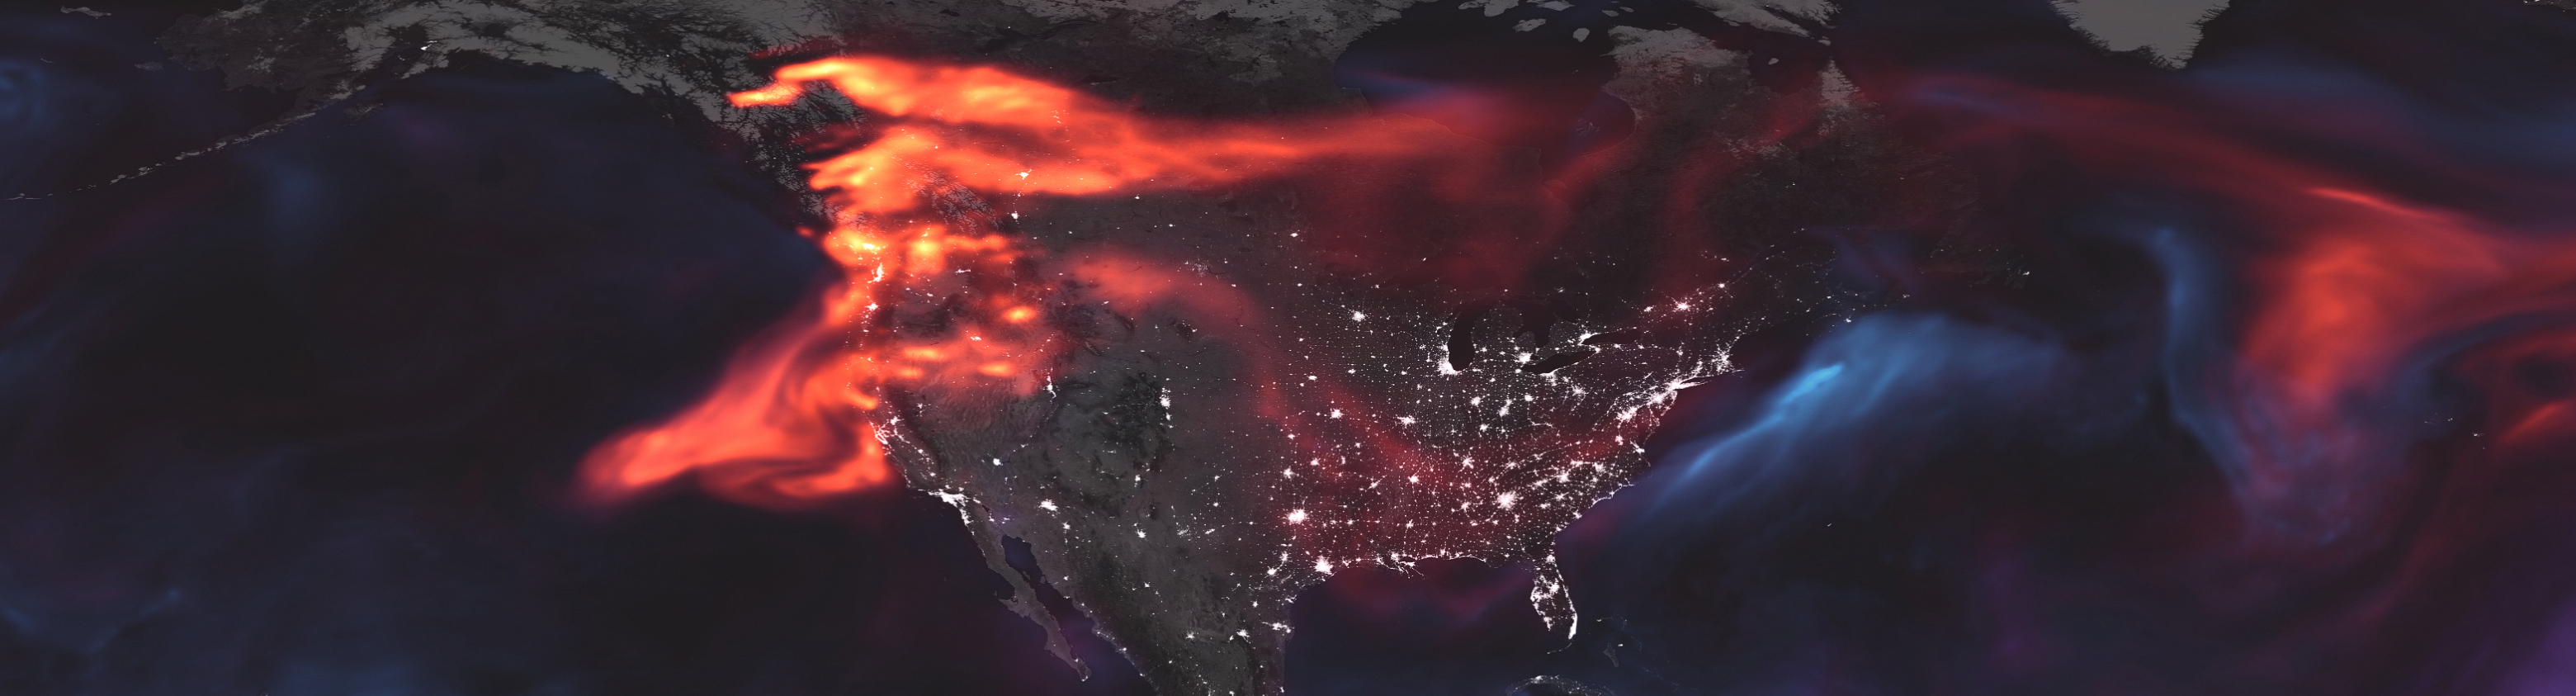
\includegraphics[width=\textwidth]{images/remote_sensing/aerosols_cropped.jpg}
  \caption{A visualization of aerosols over North America on August 23, 2018, using output from NASA's Goddard Earth Observing System Forward Processing model. Black carbon (red) in this image is primarily due to wildfires in the United States and Canada; it can also be emitted by vehicles and factories. Image Credit: NASA/Joshua Stevens/Adam Voiland.}
  \label{teaser}
  \end{figure*}
  
\subsection{Remote Sensing and Analysis}
There has been much research on approaches to analyzing wildfire-related data, though few approaches are practically applicable to real-time scenarios. The authors of~\cite{Coen2013} use remote sensing fire detection data to initialize and evaluate fire growth simulations. In such simulations, uncertainty grows over time; updating the model with the most recent satellite detections helps make sure that the model and the detections are within one another's error bounds. As with modeling fires themselves, modeling the traffic from evacuations is highly dependent on variation and uncertainty in input data. However, approaches such as dynamic traffic assessment (DTA), for planning for evacuations and related traffic, currently assume deterministic inputs, whereas whether an evacuation plan is optimal, or even possible, depends upon the confidence in the inputs~\cite{Yao2009}. (These inputs include properties like specific fire conditions,  and a fire's likelihood of moving in a certain direction.)



%…real-time….
Satellites are increasingly vital to real-time assessment of natural disasters. For one, they help provide relative certainty while ground-based information is often limited, incomplete, or inconsistent, especially during an ongoing disaster~\cite{Voigt2016}. Satellite data are especially promising for filling gaps in current modeling and prediction capabilities. Detections are often provided at more frequent intervals than perimeters, which are reported by humans observing the fire on the ground. 

% * <mvgomov@ucdavis.edu> 2018-07-16T21:09:52.262Z:
% May be worth noting that they provide relative certainty while also being provided at a more regular (& frequent) interval than "on-the-ground" data like perimeters, which are only supplied every ~6-12h (and embargoed by Calfire for some time before they're publicly released as well?) 
% 
% ^.

However, analyzing satellite data involves myriad challenges, including uncertainties from a wide range of sources, and the general difficulty of combining heterogeneous sources~\cite{Luppino2017}. Historical data are widely used to test and hone detection analysis methods. For example, the authors of~\cite{Luppino2017} use clustering analysis to identify changes among heterogeneous satellite images. Interpolated satellite data can be used in the process of making biomass estimates~\cite{Zhang2011}; this links satellite data to what has happened on the ground, to learn how to better interpret satellite data.

%how do things like clouds and smoke affect the analysis we can do of historical fires? how can we use that to help us improve responses to future fires?


Fire radiative power (FRP), estimated from satellite detections, can be used to estimate the total energy released in burning, which in turn can be used to model atmospheric emissions from a fire~\cite{Boschetti2009}. However, this process is highly sensitive to the uncertainties introduced by cloud cover, etc. Estimating the total energy released in a fire (the Fire Radiative Energy, or FRE) is of interest for modeling the atmospheric emissions due to a fire. The authors of~\cite{Boschetti2009} fuse FRP data with burned area data to provide FRE estimates; they attain promising results that are still highly sensitive to the fusion approach and the treatment of uncertainty. FRP can also be used to classify fires into distinct types~\cite{Smith2005}.

Still other applications require more precise information and improved analysis to solve, such as ``spatially and temporally explicit estimates of the quantity of biomass consumed'' in a fire~\cite{Giglio2006}. These estimates may be possible using satellite detections~\cite{Zhang2011}. There is interest in, for example, discovering the correlations between FRP and meteorological information; currently, data available from satellites are generally not detailed enough to be able to make meaningful connections in this area~\cite{Peterson2012b}. Improved tools for visual analysis of historical satellite detections, other related data, and integration with data science techniques can help improve the outlook for advanced wildfire management using satellite detections.

In this study, we present an uncertainty-aware visualization approach for assessing satellite data through several analysis steps: characterizing raw, heterogeneous detections, fusing these detections, and interpolating them. Through a set of case studies, we examine how uncertainty-aware visualization can inform this process, with the potential to improve real-time analysis of satellite fire detections and other sensor data through data science approaches.

%Primarily, our focus is on fusing heterogeneous data to make it accessible for decision-making by emergency management workers. The visualization and analysis in this process is a vital link between gathering raw data and decision-making (either from interpolated detections or from other derived information).

%The ultimate goal is to help emergency managers decide where to allocate resources in a fire, and in general, where the fire will move; this affects structures, roads, pipelines, agriculture, people, and animals.

%what’s the target audience for this? is there a scenario in which the uncertainty part will be useful for users?
%- people honing algorithms (those working on wildfire predictions, or domain experts within emergency management department
%- temp emergency management users (at the endpoint)

%We present the following contributions:
%\begin{itemize}
%\item{An interactive visualization framework for tracking uncertainty through data analysis processes, incl. fusion and interpolation}
%\item{(how much to generalize or narrow this statement?)}
%\item{goal: at each step, we understand the data and uncertainty for proper application of data analysis}
%\item{allow for evolving/varied/domain-specific understanding of what each type of detection means, and therefore how to add it to existing knowledge from other detections}
%\item{``summarize,'' quantitatively, what the satellite data is telling us, in order to put into other fire-related algorithms, etc}
%\end{itemize}

\begin{figure*}[h]
    \begin{subfigure}[t]{0.26\textwidth}
        \centering
        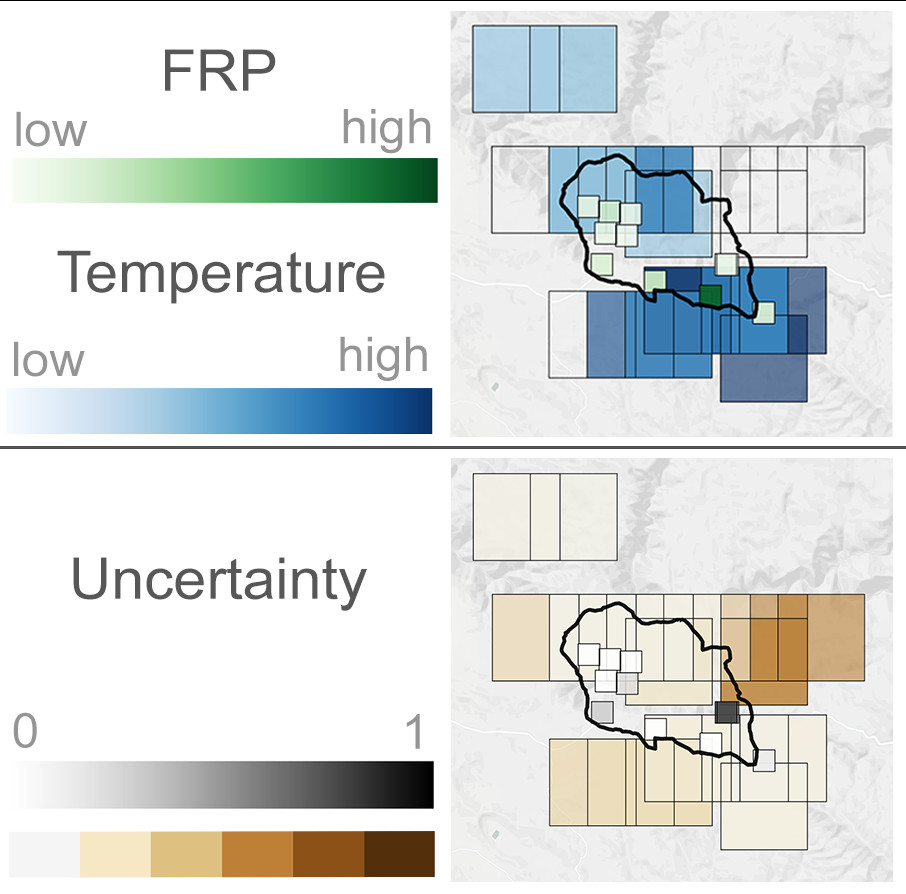
\includegraphics[height=1.6in]{images/remote_sensing/satellite_fusion_diagram_1.jpg}
        \caption{Raw detections.}
        \label{demo_1}
    \end{subfigure}\hfill%
    \begin{subfigure}[t]{0.44\textwidth}
        \centering
        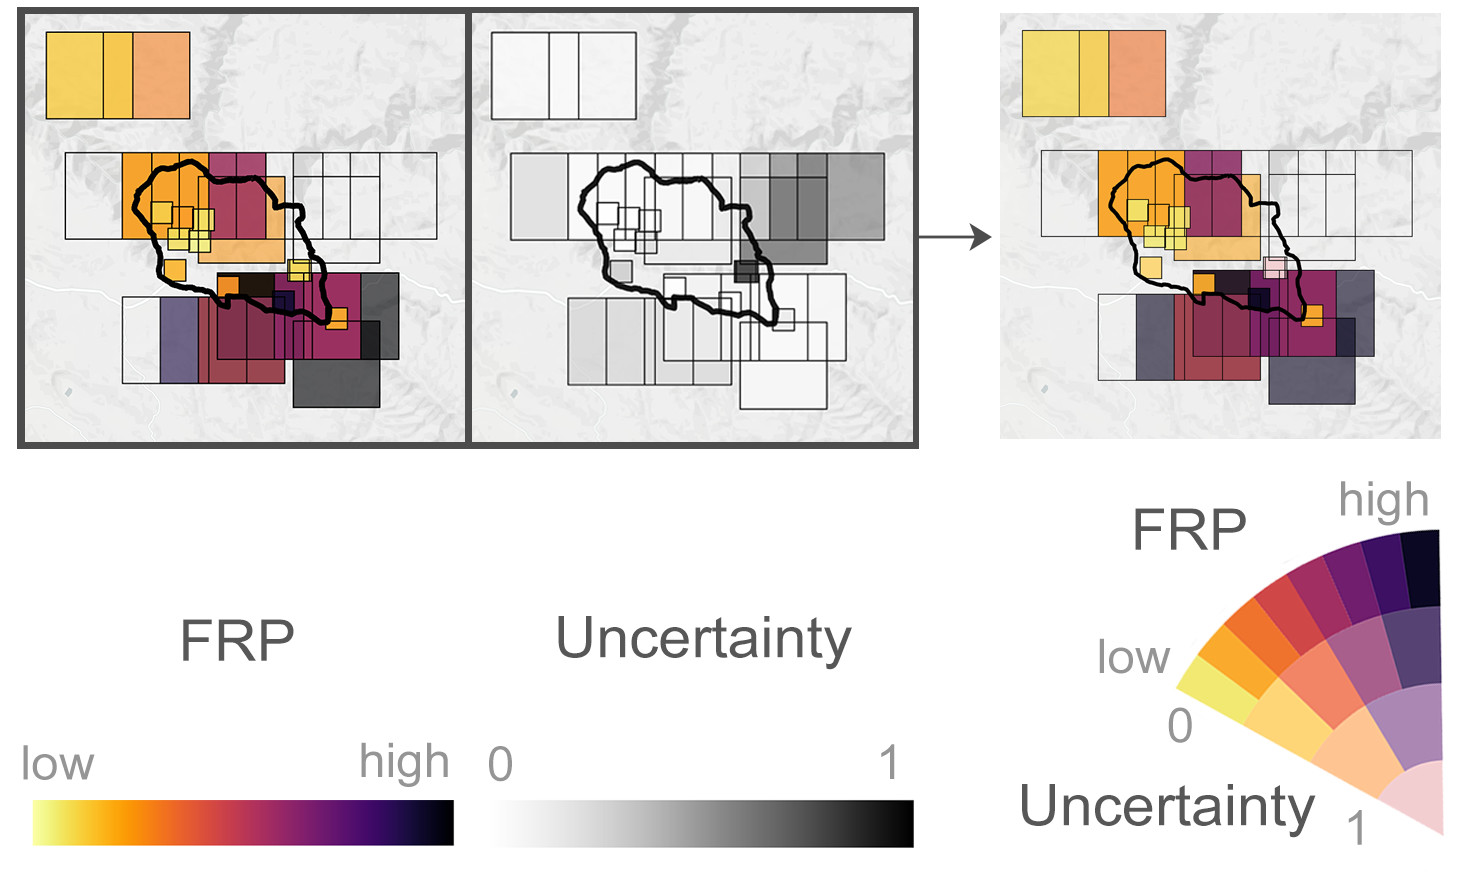
\includegraphics[height=1.6in]{images/remote_sensing/satellite_fusion_diagram_2.jpg}
        \caption{Detections and uncertainties.}
        \label{demo_2}
    \end{subfigure}\hfill%
    \begin{subfigure}[t]{0.26\textwidth}
        \centering
        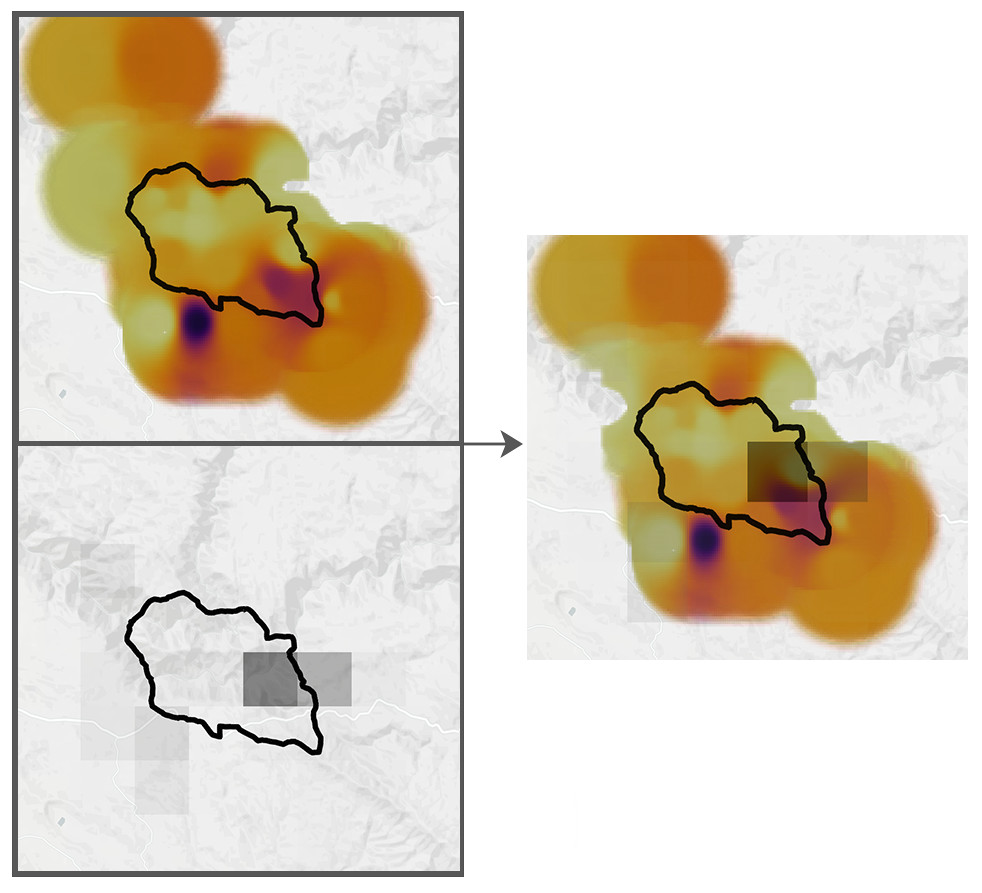
\includegraphics[height=1.5in]{images/remote_sensing/satellite_fusion_diagram_3.jpg}
        \caption{Interpolated detections.}
        \label{demo_3}
    \end{subfigure}
     \caption{Visual encodings to show uncertainty propagating through the data analysis process. \\Step 1 (a): Raw detections from GOES (larger) and MODIS (smaller). Top: FRP and temperature estimates are encoded with different scales; some GOES detections have no temperature estimate. Bottom: uncertainties for each detection, encoded with two different scales, one numerical and one categorical. \\Step 2 (b): Detections and uncertainties are each encoded into a single color scale. Note the high-uncertainty small detection on the right side of the perimeter; this corresponds with a detection showing a low FRP value amid other high detection values. At right, we use a bivariate ``value-suppressing uncertainty palette''~\cite{VSUP} to encode values and uncertainty simultaneously. \\Step 3 (c): Interpolated detections using IDW (top); corresponding uncertainties encoded in a grid (bottom). Combining these images into a single view (right), we see that the uncertainty reflected in the low-FRP detection from Figure~\ref{demo_1} is occluded by the uncertainty grid.}
     \label{summary_figure}
\end{figure*}

\subsection{Data}
We obtained data from two of the most common sources of satellite data for wildfire analysis: NASA's Moderate Resolution Imaging Spectroradiometer (MODIS) and NOAA's Geostationary Satellite Server (GOES). MODIS instruments fly on two ships, Terra and Aqua, each with a different orbit around Earth; we use detections from both. Combining Aqua and Terra data can help eliminate non-detections and decrease the uncertainty in detection rates~\cite{Hawbaker2008}. Additionally, we use detections from two GOES satellites, GOES-13 and GOES-15.

Recently, NASA and USGS have planned to combine GOES and MODIS detections, and others, in real time, to improve the tracking and documentation of fires; many historical fires are missing from state and federal records~\cite{Howard2014}. Therefore, we hope that an exploration of how to analyze these highly heterogeneous data together will be more broadly applicable to other data fusion applications.

%These instruments each have multiple sensors, and report results with different spatial resolutions, at different frequencies, with different measurements and uncertainties. 

%FRP, detections, resolution

%\item{talk about the wide range of uncertainties in the data}
%\item{for example, what does information about what a satellite footprint actually tell us vs. what we need to know? — how likely is the actual detection to be in any part of the footprint? what can we deduce outside the footprint?}


%~\cite{Giglio2006} MODIS can be used to estimate burned area after a fire,,,
%talk about measurements and uncertainties
The GOES detections we obtained have a resolution of 4km, while the MODIS detections have a 1km resolution. GOES provides a temperature estimate if possible, as well as an uncertainty class, such as ``high confidence fire pixel'' or ``saturated fire pixel'' (for more detail, see~\cite{nesdis2010goes}).
MODIS estimates FRP using the temperature, as in~\cite{Freeborn2014}. This calculation introduces uncertainty into the reported value of FRP, especially due to variation of the actual detection location within a satellite pixel.

These detections and estimated temperature and FRP values include uncertainty primarily resulting from cloud cover, smoke cover, and saturation.
There are uncertainties in MODIS detection rates, which makes it hard to accurately interpret statistics derived from detections~\cite{Hawbaker2008}.

FRP is a good characterization of fire intensity~\cite{Peterson2012b}. However, FRP alone is simplistic; for example, an FRP value could be equal for two pixels in different scenarios, such as a large fire with low intensity or a small fire burning with high intensity~\cite{Peterson2012a}. To supplement this information, some high-confidence detections also contain sub-pixel estimates for temperature; we ignore these in this study.

In this study, we consider historical data, but with an aim toward data analysis that could be performed in real time. Additionally, historical study is important on its own. For example, to study and improve decision-making, emergency management workers use historical weather data in simulated scenarios because of the difficulty in simulating weather~\cite{Baumgart2006}. Similarly, modeling fires and weather's effect on fires is difficult, so studying historical fire data (especially in conjunction with historical weather data) is important.

\begin{figure}[t]
    \begin{subfigure}{0.48\textwidth}
        \centering
        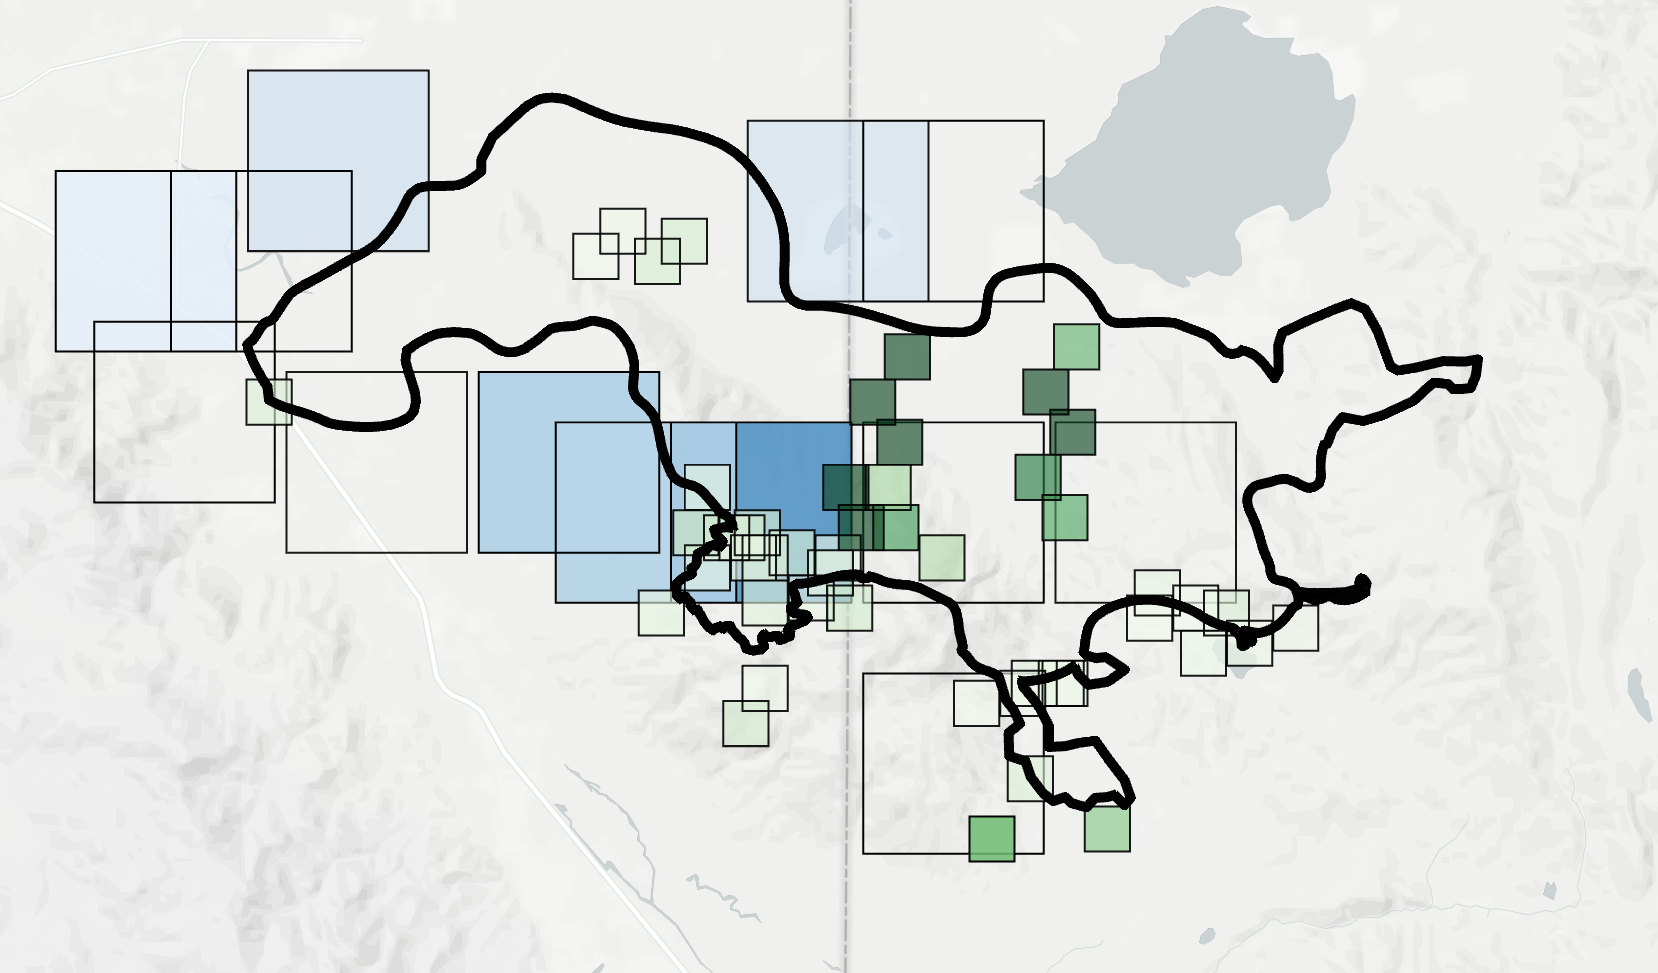
\includegraphics[width=\textwidth]{images/remote_sensing/step_1_example.png}
        \caption{Detections from GOES (temperature mapped to blue) and MODIS (FRP mapped to green) for one 12-hour span. The corresponding perimeter is overlaid.}
        \label{raw_detections}
    \end{subfigure}
    \begin{subfigure}{0.48\textwidth}
        \centering
        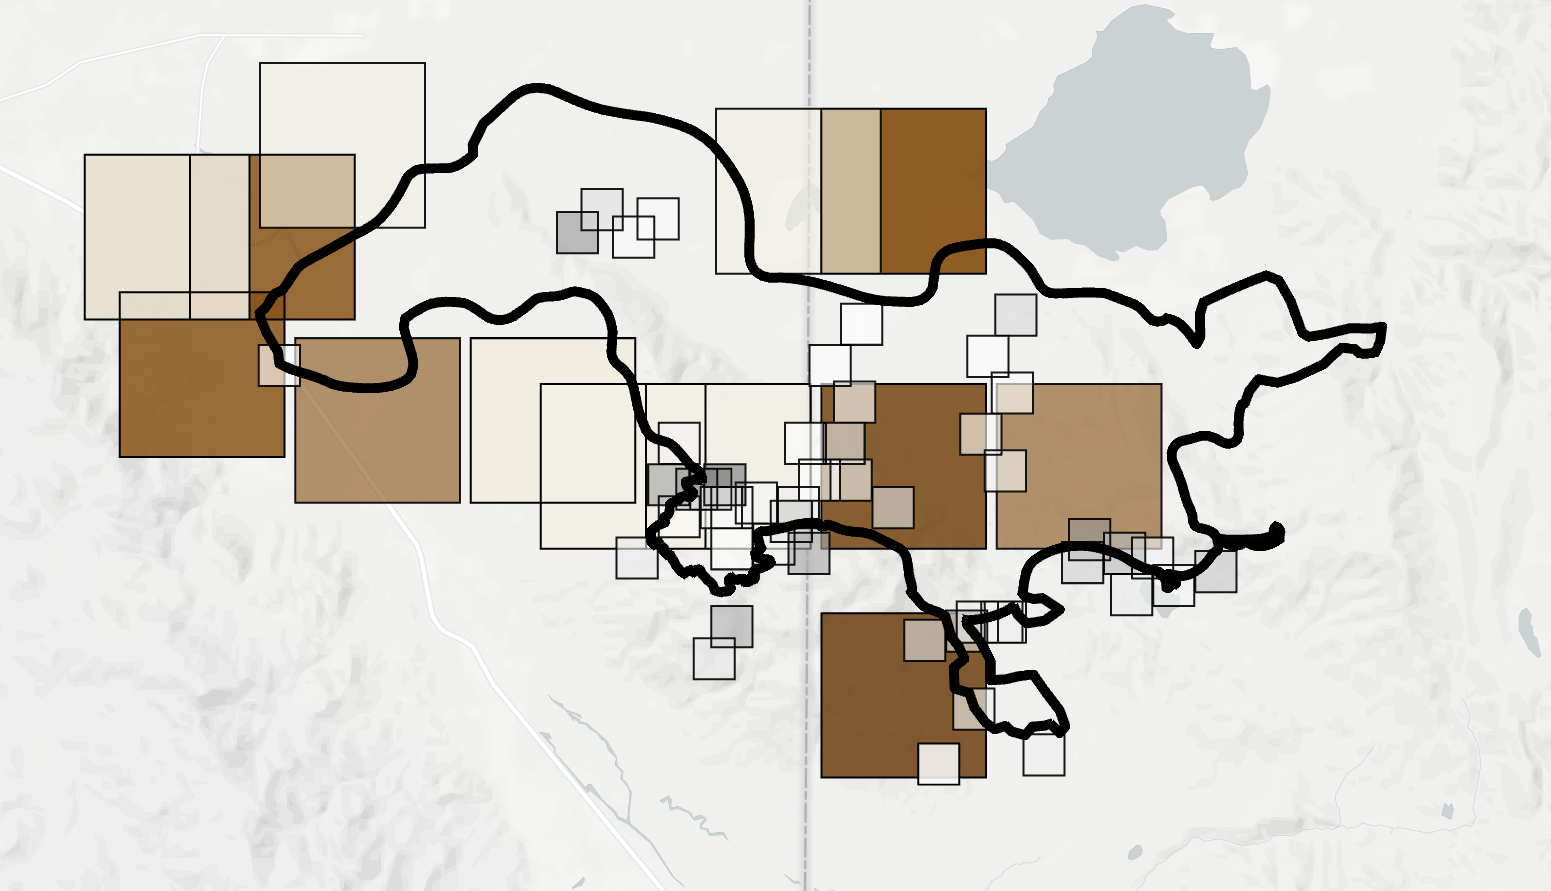
\includegraphics[width=\textwidth]{images/remote_sensing/step_1_uncert.png}
        \caption{Uncertainties from GOES (brown) and MODIS (gray) detections corresponding to Figure~\ref{raw_detections}. Note that GOES footprints can have a confidence level without a corresponding temperature estimate.}
        \label{raw_uncertainty}
    \end{subfigure}
     \caption{Satellite detections and uncertainties for the Long Valley fire in California and Nevada for the last twelve hours of July 14, 2017. The color mappings used are introduced in Figure~\ref{demo_1}.}
     \label{assess_detections}
\end{figure}

\section{Methods}
\label{methods_section}
The primary steps in our analysis are:
\begin{enumerate}
\item{Assess raw (heterogeneous) data}
\item{Fuse data}
\item{Interpolate and analyze data}
\end{enumerate}

\noindent In each step, uncertainty is involved, growing with each transformation. According to~\cite{Pogson2015}, ``the effects of combining aggregated spatial data are found to obey standard properties of error propagation,'' including for resolution-related uncertainty. We employ standard error propagation as appropriate in our calculations. These steps are shown in Figure~\ref{summary_figure}. Before describing our visualization approach, we outline each step in more detail.

\subsection{Assessing Detections}
In this stage, we note that some of the GOES detections have no temperature estimates, but they still have uncertainty values (see Figure~\ref{assess_detections}). We can use this information as desired in the next steps. We can also note areas where detections from different satellites seem to show quite disparate information, and determine whether reported uncertainty explains the discrepancies.  

\subsection{Fusing Data}
Merging multiresolution, multiple-sensor data has several possible approaches, including principal component analysis and high-pass filtering~\cite{Chavez1990}. In our case, there is generally only one value per detection, as opposed to image data, so we use simpler approaches.

First, we would like to merge temperature estimates and fire radiative power (FRP) estimates into a single numerical scale. Temperature and FRP are theoretically related by the Stefan-Boltzmann relationship~\cite{Peterson2012a}:
\begin{equation}
FRP = \sigma(T^4 - T_b^4)A_f
\label{frp_eqn}
\end{equation}
where $\sigma$ is the Stefan-Boltzmann constant, $T$ is the detected temperature, $T_b$ is the background temperature, and $A_f$ is the detected area. In practice, calculating FRP from temperature is complex due to subtleties in determining the background temperature and detected area~\cite{Xu2010}. To measure FRP for individual pixels retrieved by MODIS, a best-fit equation is employed~\cite{Peterson2012a}. For our proof-of-concept, we provided a rough estimate for the conversion between temperature and FRP for GOES detections. Equation~\ref{frp_eqn} could include propagation of uncertainty from the temperature values, but because this is a rough estimate, we do not think it would be meaningful to calculate uncertainty this way at this stage. Figure~\ref{fuse_detections} shows a fused result which we can use to check that the temperature scaling makes sense.

At this stage, we also combine the reported detection uncertainties into a single numerical scale. (We do not yet take uncertainty from multiple resolutions into account.) Detections from MODIS rank uncertainties on a 0-100 scale, while GOES provides categorical designations. To convert between the two, we assign a numerical value to each category (for example, ``medium possibility fire pixel'' = 70, ``high possibility fire pixel'' = 90, ``partially cloudy/smoke fire pixel'' = 30). We can use a fused view to check that these uncertainties are somewhat consistent with one another. Most will be particular to their satellites, but external uncertainties such as cloud or smoke cover should have a similar effect on all detections.

\begin{figure}[h]
     \centering
    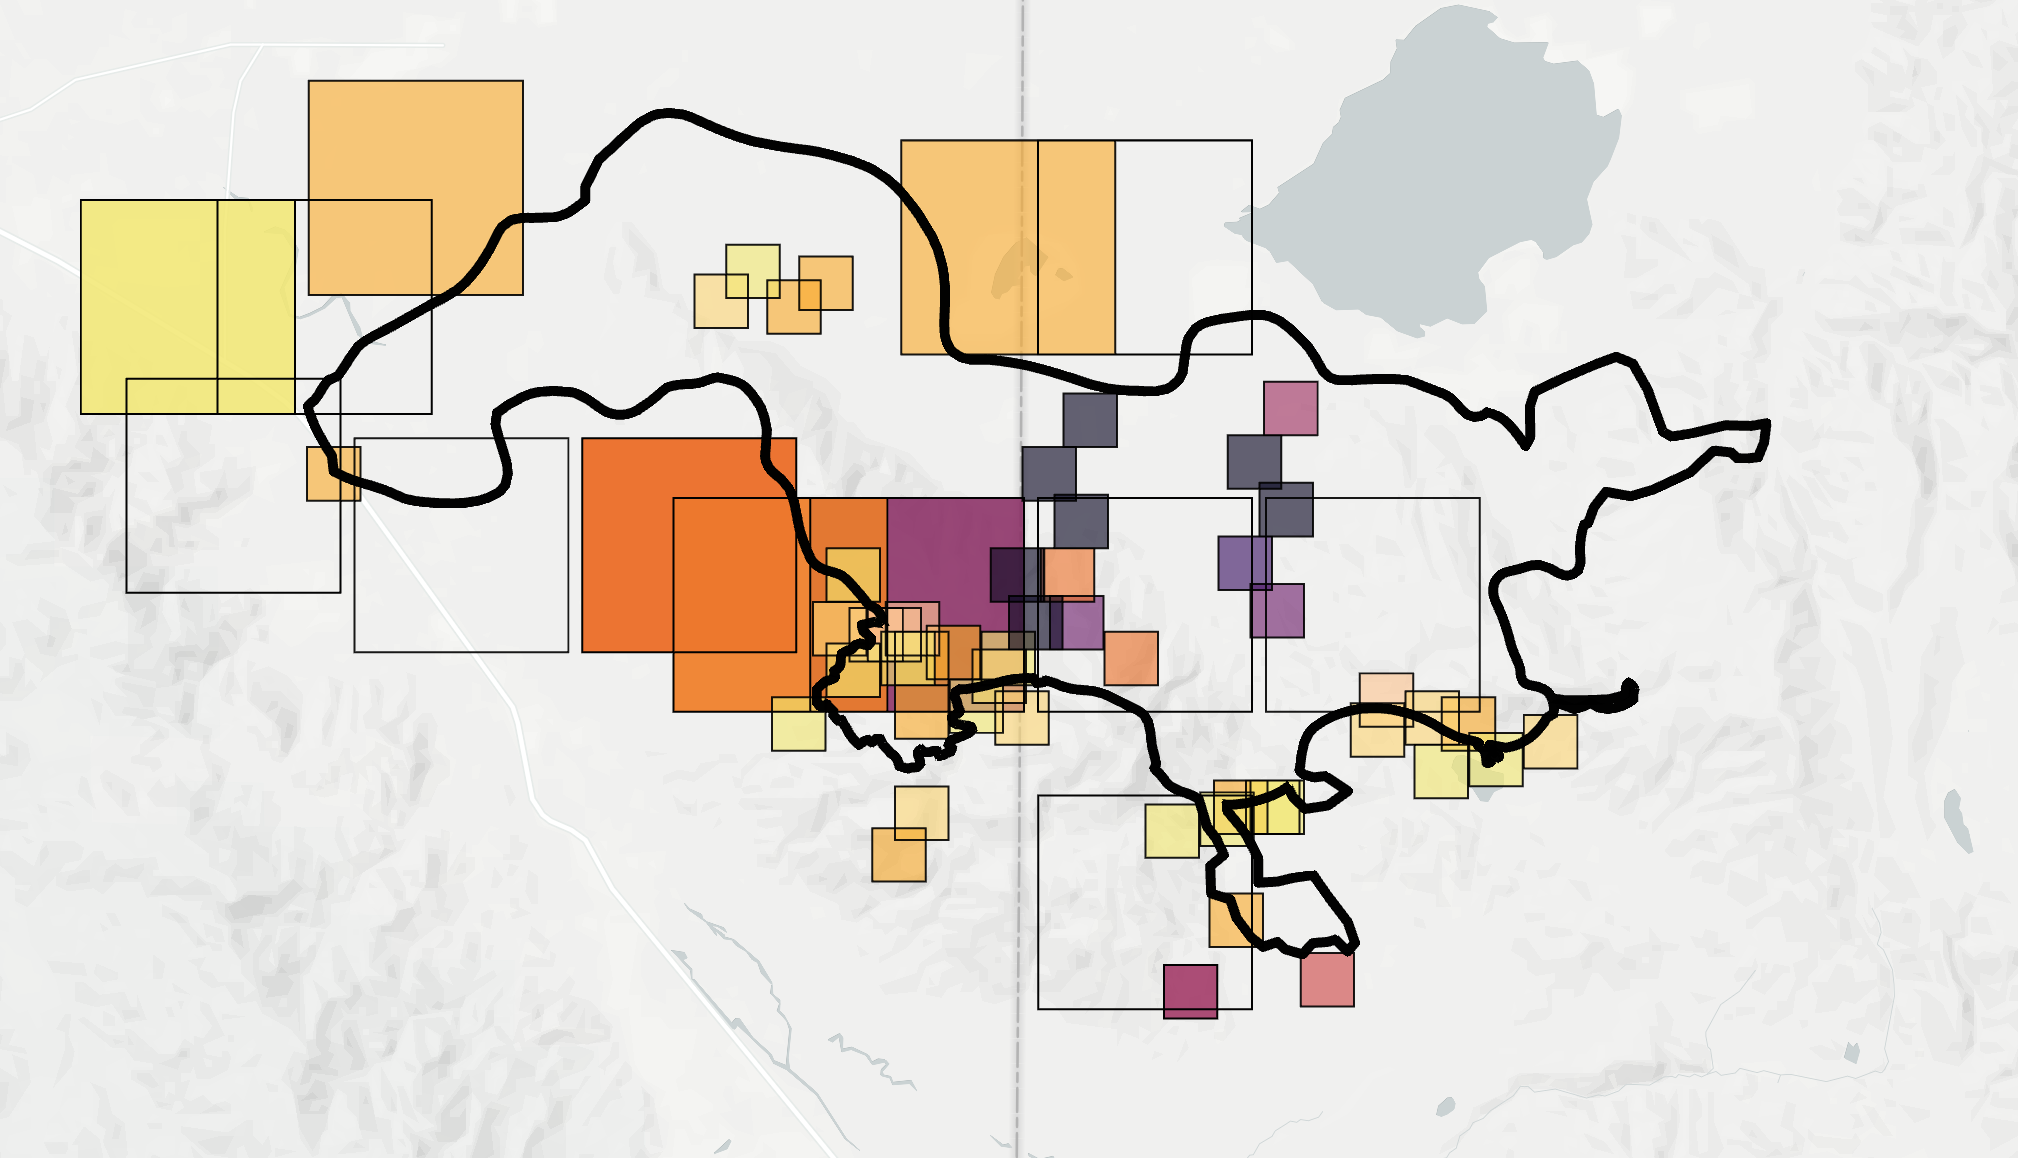
\includegraphics[width=\textwidth]{images/remote_sensing/step_2_example.png}
     \caption{Fused satellite detections and uncertainties for the Long Valley fire, corresponding to data in Figure~\ref{assess_detections}. The VSUP~\cite{VSUP} color mapping used is shown in Figure~\ref{demo_2}.}
     \label{fuse_detections}
\end{figure}

If we combine uncertainty and value (see Section~\ref{visualization}), we must decide what to do with footprints that have no corresponding temperature. Perhaps they can increase the confidence of any other nearby detections if their confidence is relatively high. However, Figure~\ref{raw_uncertainty} shows that the low-confidence GOES detections correspond to those without a temperature estimate, so ignoring these data is also a viable option.

\subsection{Characterization and Analysis}
%The ambiguity introduced by the steps above introduces ambiguity into interpolated outcome.
%how does IDW treat uncertainty ``the right way'' ?
Next, we use data analysis to characterize the satellite detections over a time window. 
\subsubsection{Inverse Distance Weighting}
One approach is to use interpolation techniques to estimate values for points over a smoothed region. Interpolation has been successfully used to supplement incomplete fire information with satellite detection data, such as mapping the day-to-day progression of burning~\cite{Parks2014}. Here, interpolating the timing of satellite detections can make up for the fact that fire perimeters are often incomplete or unavailable. The author of the day-of-burning study compared ten interpolation techniques and found that variations of Weighting by Mean and Distance (WMD) and Inverse Distance Weighting (IDW) provided the best results; however, uncertainty was not taken into account, and no confidence levels were assigned to the predicted values.

In IDW, values are calculated using:

\begin{equation}
V(x) = \frac{\sum_{i=1}^{n}w_i(x)v(x)}{\sum_{i=1}^{n}w_i(x)}
\end{equation}

where the weight is based on the inverse of the distance to some power, $p$:
\begin{equation}
w_i(x) = \frac{1}{\mathrm{dist}(x, x_i)^p}
\end{equation}

IDW can weight either the $n$ nearest neighbors or those within a radius $r$. The latter gives us smoother results. It also makes more sense for this application: our intuition says that detections probably have meaning within some consistent radius, maybe related to their spatial resolution.

Using standard error propagation, we calculate how uncertainty in each detection contributes to uncertainty in the interpolated value:

\begin{equation}
    \sigma_v = \frac{\sqrt{\sum_{i=1}^{n}(w_i
    \sigma_{v_i})^2}}{\sum_{i=1}^{n}w_i(x)}
    \label{idw_uncert}
\end{equation}

To use the result in Equation~\ref{idw_uncert}, we need to know the standard deviation of each temperature or FRP measurement, $\sigma_{v_i}$, but instead, we only have the reported confidence levels or categories, which do not have a clear association with standard deviation. One approach is to supply an estimate of the relative standard deviation, $\sigma_{v_i}/v_i$, for each confidence level. In this application, we are concerned with relative confidence in the measurements, rather than a precise  range of possible values for each measurement, so we propose that this approximation is sufficient for understanding the propagated effect of uncertainty in the measurements.

We could also include the propagated effect of errors in the distances used, as in~\cite{doi:10.1080/10106040801966704}. This would significantly complicate the error calculation. Additionally, there is not a clear way for us to measure the error in the distance between each detection and the sample position. One interpretation could be to assign more uncertainty to lower-resolution satellite detection footprints, indicating that these data provide less precise information about position than do high-resolution footprints. In this study, we choose to assume no error in the sample distances, using only the centroid positions provided for input into the IDW algorithm.

%Kriging is another possible approach to interpolating the detections over an area.

%want to keep original data available (i.e. frp for hovered-over points)
\subsubsection{Kernel Density Estimation}
For our second approach to characterizing satellite detections, we use kernel density estimation (KDE). KDE estimates the probability density function, $f(x)$, of a variable (in this case, FRP):

\begin{equation}
f(x) = \frac{1}{nh}\sum_{i=1}^{n}K(\frac{x-x_i}{h})
\end{equation}

where $K$ is the kernel, and $h$ is the \textit{bandwidth}, which determines how wide a radius
to smooth values over. In this study, we use a Gaussian kernel.

%which kernel do we use?
%how can/does KDE take uncertainty into account?

With this approach, we hope to identify, roughly, the likeliest new and ongoing fire activity around the perimeter. KDE does not put out an uncertainty value; instead, the uncertainty is encoded within the result itself. That is, detections with higher uncertainty are assigned lower weights. Therefore, we can inspect uncertainty through the rest of the pipeline, leading up to performing KDE, to assess whether it looks like uncertainty information has been properly incorporated.
%briefly weighting

%how does it take reference and target time into account?

%can i weight the more recent detections more heavily?

\subsection{Visualization Approach}
\label{visualization}

As much as possible, our encodings should be ``informationally equivalent'' throughout the data analysis steps, which is difficult because uncertainty introduces a lot of complexity and clutter to maps~\cite{Kinkeldey2014b}. Ideally, adding more information to an image should not look like ``more fire'' is being added, just that we are more certain about the information that is there. Above all, our encodings should be intuitive to someone without much specialized knowledge. While emergency managers such as our collaborator have extensive knowledge of fire-related data, during an ongoing event, workers who do not have specific emergency management expertise may be brought in; any tool supporting decision-making with visual analysis should be easily accessible to them. The visualization approaches we use are summarized in Figure~\ref{summary_figure}.

In a survey of geospatial-uncertainty-related user studies~\cite{Kinkeldey2014b}, the authors identify three main dichotomies: intrinsic/extrinsic; coincident/adjacent; static/dynamic. We explore these axes to apply the appropriate uncertainty visualization mode for each step in our data analysis.
 
No significant distinctions are found between coincident and adjacent approaches~\cite{Kinkeldey2014b}. Here, we aim for coincident when possible (i.e., when the information is reduced enough for meaningful coincident encodings); it seems easier on the mental map. Most approaches surveyed used static images rather than dynamic, animated approaches. For simplicity, we focus on static images representing a chosen time window.

\begin{center}
    \begin{tabu} {p{2.2cm}|p{10cm}X[l]}
          Coincident & Use if possible: easier for the mental map\\
          \midrule
        Adjacent & Use if there is too much information to meaningfully include with data 
    \end{tabu}
\end{center}

For intrinsic uncertainty depiction, the authors find that from the studies surveyed, hue, value, and transparency are best for conveying uncertainty (with darker representing higher uncertainty being most effective)~\cite{Kinkeldey2014b}. The Value-Suppressing Uncertainty Palette (VSUP)~\cite{VSUP} creates a bivariate map for encoding value-uncertainty combinations (see Figure~\ref{summary_figure}). One goal of this approach is to improve decision-making by making it harder for the user to distinguish between uncertain states, and easier to make precise distinctions when uncertainty is low. 

\begin{figure*}[h]
    \begin{subfigure}[t]{0.5\textwidth}
        \centering
        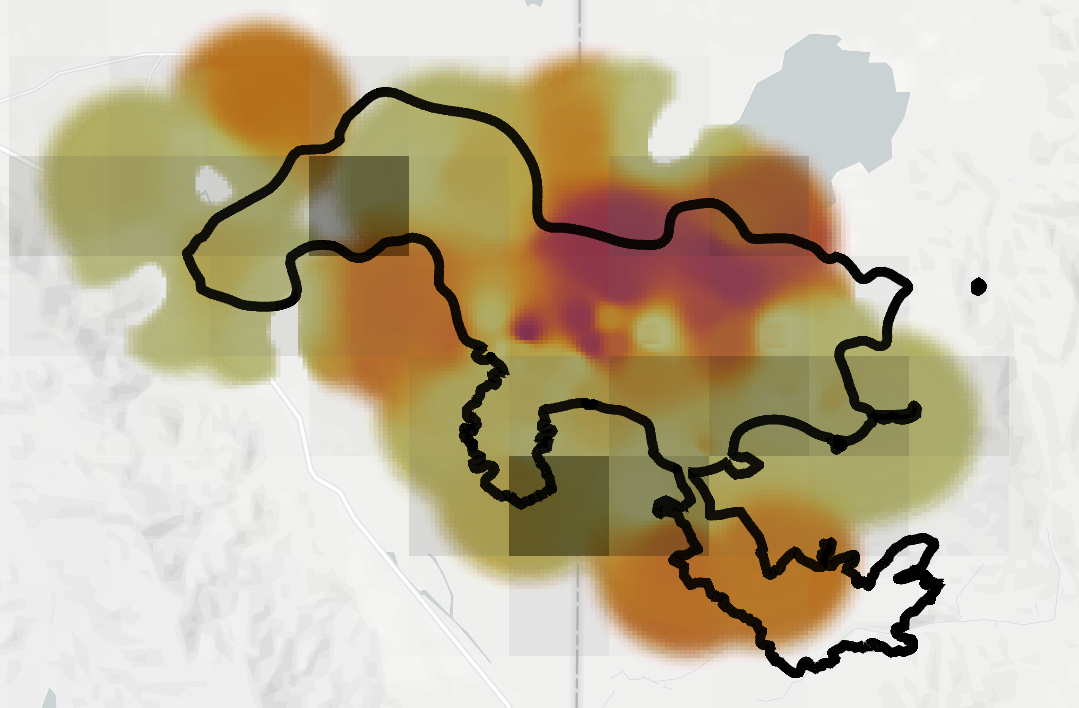
\includegraphics[height=2in]{images/remote_sensing/idw_casestudy_p4_r3_5.png}
        \caption{IDW results with $p=4$, $r=3.5\mathrm{km}$. The next available perimeter is overlaid.}
        \label{idw_result_1}
    \end{subfigure}
    \begin{subfigure}[t]{0.48\textwidth}
        \centering
        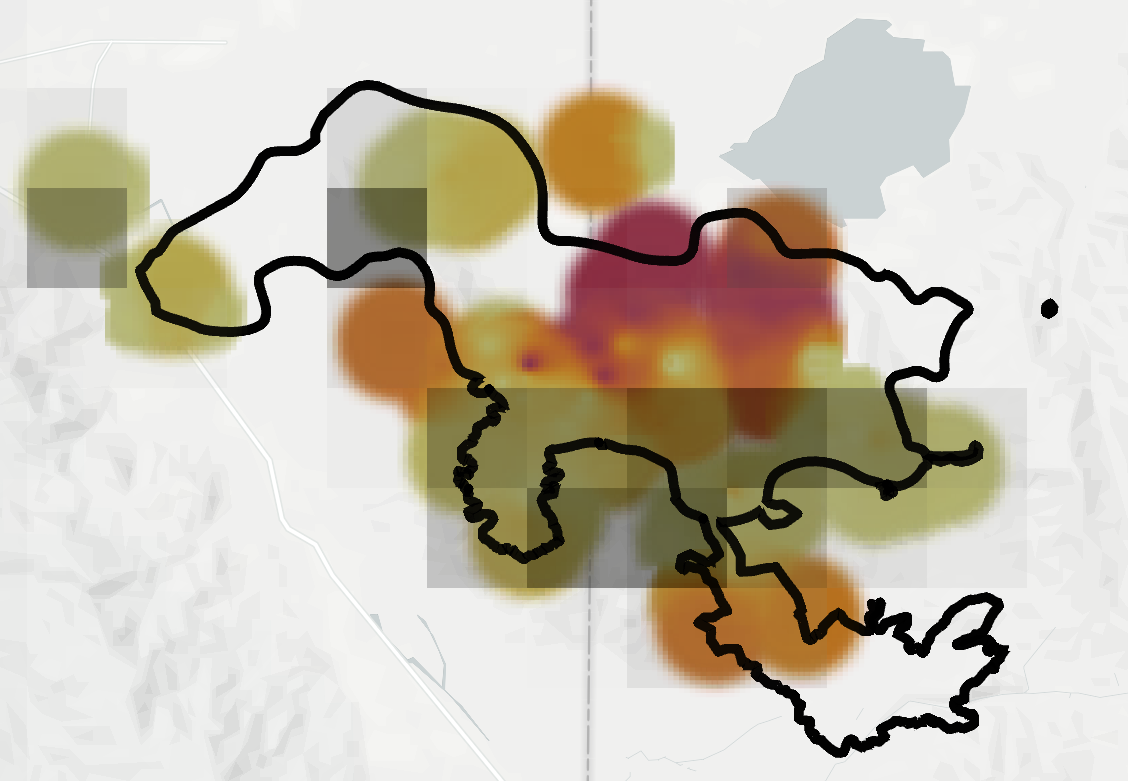
\includegraphics[height=2in]{images/remote_sensing/idw_casestudy_p2_r1_8.png}
        \caption{IDW results with $p=2$, $r=1.8\mathrm{km}$. The next available perimeter is overlaid.}
        \label{idw_result_2}
    \end{subfigure}
     \caption{Using Inverse Distance Weighting to characterize fire behavior. The color map (non-VSUP version) is introduced in Figure~\ref{demo_2}, with yellow corresponding to lower activity and purple corresponding to higher activity.}
     \label{idw_ref}
\end{figure*}

%``there’s a limited budget for perceptual discriminability''

%quantization error vs. perceptual error
Extrinsic techniques are used in fewer of the studies surveyed in~\cite{Kinkeldey2014b}, but are recommended in cases where color is already used to depict values, such as in map-based visualizations~\cite{Kinkeldey2014a}. The authors of~\cite{Kinkeldey2014a} implement grid-based uncertainty for maps using lines depicted with varying amounts of visual noise. They find that how users perceive the uncertainty depends strongly on the number of levels. This can be ameliorated somewhat by maximizing relative differences between encodings, but complex ``mixed'' uncertainty information, as in our application, makes this hard. Grid-based methods can also vary the size of the grid to indicate uncertainty level, such as using a tessellated quadtree in~\cite{Kardos2007}.

\begin{center}
    \begin{tabu} {p{2cm}|p{8cm}X[l]}
        Intrinsic & Use when uncertainty is a property of each item \\
        \midrule
        Extrinsic & Use when uncertainty is more accurately defined over a region  \\
    \end{tabu}
\end{center}

We use intrinsic methods to depict satellite detections, but switch to a grid-based visualization once the data are interpolated, because this step introduces more complex color encoding. Because the interpolated images are complex, we aim for a simpler grid-based uncertainty visualization than the examples above. Our implementation includes a grid with cells of fixed pixel size, showing more detail as a user zooms in. Each cell is colored with a grayscale value corresponding to the aggregated relative interpolated uncertainty in that area (see Figure~\ref{demo_3}).

%discuss:
%- smoke analogy (grid-based method!) doesn’t make sense for the individual detections, since superimposing a grid would be arbitrary.
%- another principle we use: one scale (color) per unique data scale; this goes for values and their uncertainties.
%- what does each view/encoding show us?
%talk about the use of opacity: here, to (kind of) indicate uncertainty in the %``where''

%**NOTE that, when we fuse data and some footprints have a confidence value but no measurement value, it’s hard to depict faithfully in the VSUP

%used a perceptually uniform color scale, which seems to make the best VSUPs
%additionally, we should be visualizing `what’ and `where’ for our selected time window; in this step, `where’ gets a lot more uncertain.)

\subsection{Validation}
Quantifying success for an IDW or KDE result is difficult for several reasons. One simple approach is to compare interpolated fire activity with changes in perimeters. However, we are not making predictions, only summarizing the detected activity. Therefore, there is no ``ground truth'' to compare to. Whether the important features are captured may require expert users to determine. Additionally, perimeters are often made available significantly later (12-14 hours) than the time they reflect, so comparison with perimeters will be especially limited in real-time analysis.

However, there are varying degrees of success, and the summary does not need to be perfect to be helpful. According to our primary emergency management collaborator, knowing the direction of the fire and which general areas to send supplies to are some of the most important factors for rapid decision-making. We can rely on visual analysis to see whether our results accurately reflect
the relative levels of activity within a fire. For visual comparison, we obtain historical fire perimeters from the Geospatial Multi-Agency Coordination (GeoMAC) (www.geomac.gov).

For more thorough validation, we plan to survey emergency management practitioners in a future study, assessing how our visualization approach would impact their decision-making in historical wildfire scenarios. 

\section{Case Studies}
The case studies focus on the Long Valley Fire in California and Nevada during July 2017.

%\subsection{Fusion} 
%do uncertainties have good agreement? (i.e. clouds/smoke have clear patterns?)
%External sources of uncertainty, such as clouds or smoke obscuring satellite detections, should consistently affect observations from both MODIS and GOES satellites. Where images of the fused data agree on areas of high uncertainty, clouds or smoke may be the cause. Disagreements in the fused image, however, likely originate from other causes (see Figure ??). Adjusting the uncertainty scalings, and inspecting the resulting fused visualization, can inform how to interpret the satellite detections. [for example, ... ]

\subsection{Interpolation}
\label{interpolation}

Uncertainty-aware visualization can help improve the algorithms we use to interpolate the detections. One set of detections and their uncertainties are shown in Figure~\ref{fuse_detections}. There are three areas of activity in the lower right part of the current perimeter. The middle cluster contains detections from two different satellites, though the lower-resolution detection is also highly uncertain. The middle and right clusters each contain 6-7 higher-resolution detections with roughly similar, low uncertainty distributions. The left-most cluster contains the most detections from both satellites, with fewer low-confidence detections. Additionally, two medium-high confidence detections from one satellite lie outside the current perimeter near the cluster. 

An IDW interpolation of these detections, with the next available fire perimeter, is shown in Figure~\ref{idw_result_1}.  Of the three clusters identified near the perimeter in the first timestep, the left two turned out to indicate areas where the fire was expanding. Analyzing this outcome can help us optimize an interpolation of these data to be as informative as possible.

\begin{figure}[h!]
    \begin{subfigure}{0.48\textwidth}
    \centering
    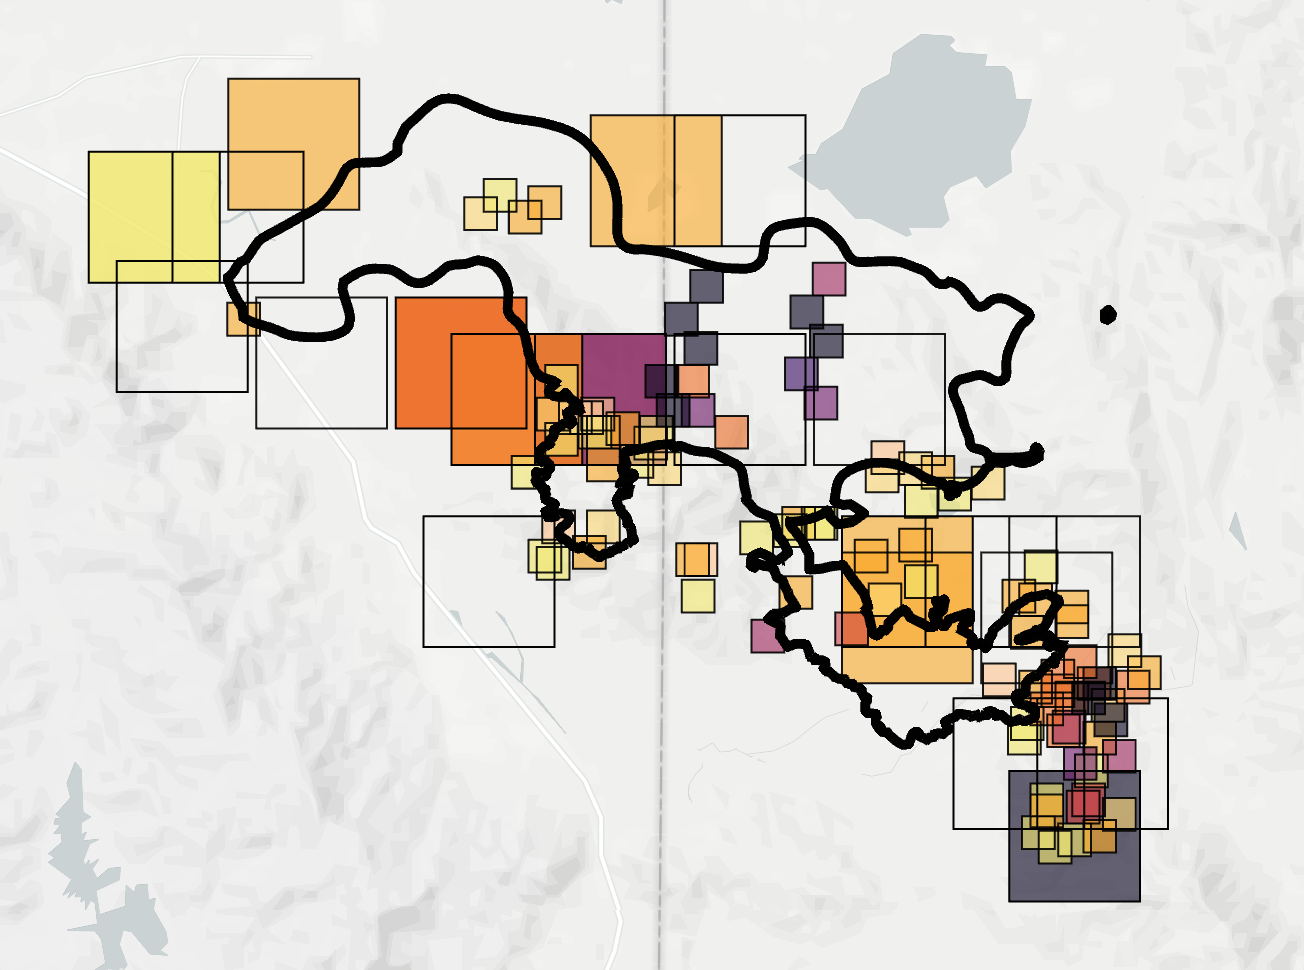
\includegraphics[width=\textwidth]{images/remote_sensing/kde_reference.png}
    \caption{Detections (with uncertainty encoded using a VSUP~\cite{VSUP}) for a later 12-hour span of the Long Valley fire.}
    \label{kde_ref}
    \end{subfigure}
    
    \begin{subfigure}[c]{0.48\textwidth}
    \centering
    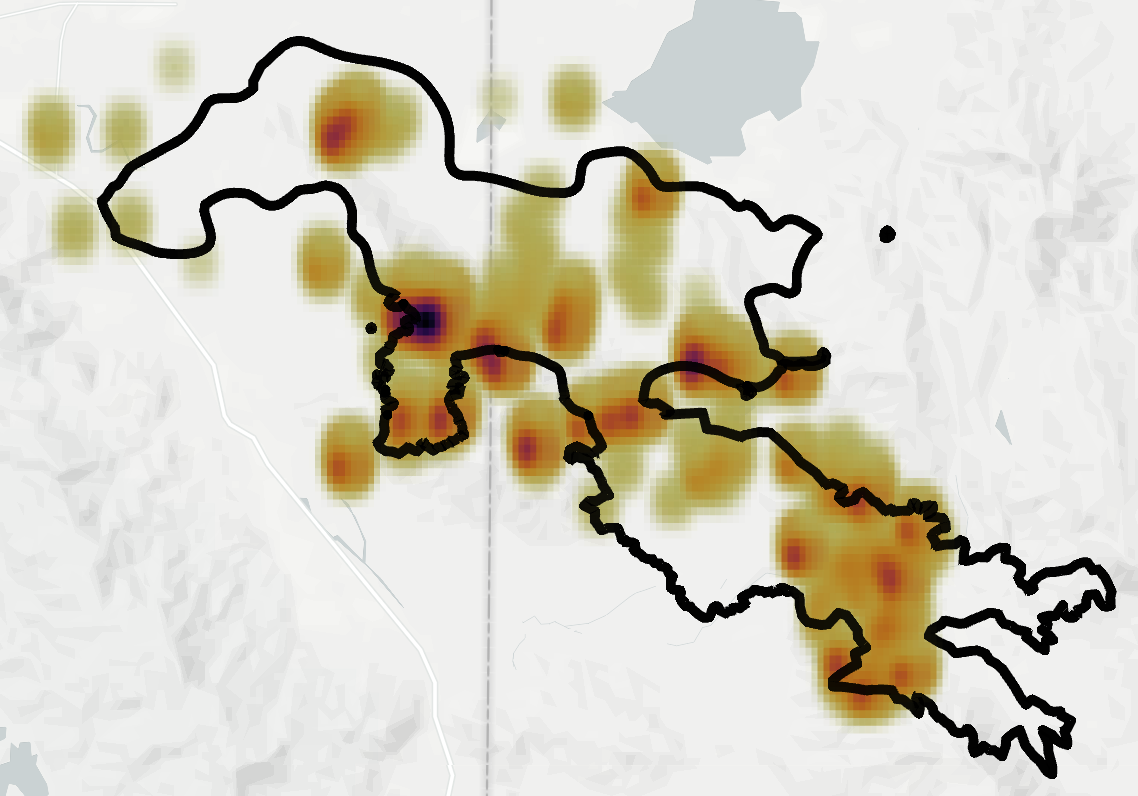
\includegraphics[width=\textwidth]{images/remote_sensing/bandwidth_a_next.png}
    \caption{KDE result showing the areas of heaviest activity. The next available perimeter is overlaid, showing the fire extending southeast.}
    \label{kde_a}
    \end{subfigure}
    
    \begin{subfigure}[c]{0.48\textwidth}
    \centering
    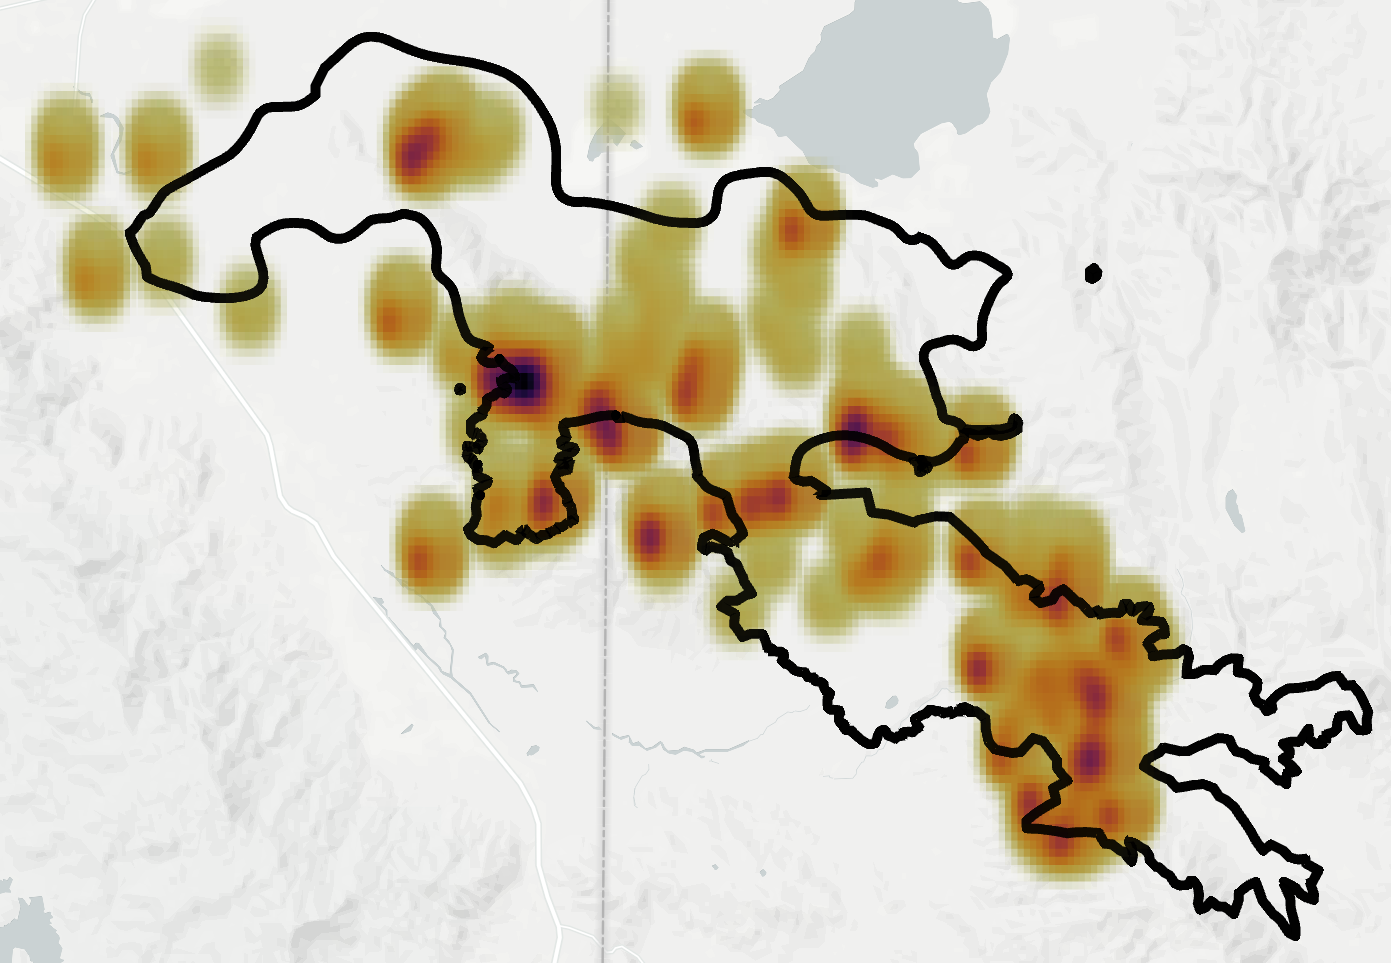
\includegraphics[width=\textwidth]{images/remote_sensing/adjusted_next.png}
    \caption{Adjusted KDE result to reflect ``smoothing'' the influence of the lower-resolution detections. This result more strongly predicts the fire's spread south and east.}
    \label{kde_b}
    \end{subfigure}
    \caption{Using Kernel Density Estimation to characterize fire behavior.}
\end{figure}

First, both of the leftmost clusters are somewhat loosely distributed, whereas the rightmost one is tightly centered on the existing perimeter. This tells us that perhaps more uncertain detections should ``spread'' their values over a larger radius than more certain detections do, but with less confidence. Also, maybe having one detection slightly beyond the border of the rest of the cluster is indicative of more movement. Because the detections in the right-most cluster were entirely in a tight group with relatively high confidence, the interpolated result should show a lower probability that those detections indicate spreading.

An adjusted interpolation result is shown in Figure~\ref{idw_result_2}. This result puts less emphasis on potential spread to the east, and indicates more variability in the detections that indicate expansion to the south. As opposed to the first result in Figure~\ref{idw_result_1}, analysts looking at this interpolation might not focus as many resources to the east side of the fire, and might focus more on the volatility in the southern direction.

\subsection{Density and Multiple Resolutions}
\label{kde}
We explore the use of Kernel Density Estimation (KDE) to find the areas of highest activity. For reference, the detections we analyze here appear in Figure~\ref{kde_ref}. The KDE calculation considers uncertainty by adjusting detection weights according to relative confidence levels. The result of one KDE implementation is shown in Figure~\ref{kde_a}. For example, the two faint orange, large footprints at the top of Figure~\ref{kde_ref} indicate low confidence, and accordingly, they are encoded as relatively insignificant in the KDE result. 

However, this approach only considers detection uncertainty, not the uncertainty that arises from combining detections with multiple resolutions. One way to address this in the KDE algorithm might be to scale the GOES (i.e., larger footprint) confidence values slightly downward, indicating that for these detections, we are less sure about the exact positions of their influence. The result of this uncertainty scaling adjustment is shown in Figure~\ref{kde_b}. The difference is subtle, but the adjusted scaling creates stronger emphasis on the southeast portion, where the fire growth is most extreme. (Another way to incorporate uncertainty from multiple resolutions, not shown here, might be to increase the bandwidth of the kernels corresponding to lower-resolution footprints.)

To continue fine-tuning the uncertainty encodings, one could use the separate and fused uncertainty views (Figures~\ref{demo_1},~\ref{demo_2}) to check how much the scaling is warping the underlying data. 


\section{Conclusions}
In order to move toward the goal of vastly improving satellite-assisted emergency management, we need to advance the capabilities of data mining and big data analysis platforms for geographical data~\cite{Voigt2016}. Applying data science techniques to sensor data, though, is fraught with difficulties, including (but not limited to) uncertainty. Visual analytics, using an approach like ours, could provide a helpful tool as data scientists and emergency managers work together to improve analytic and predictive capabilities from satellite (and other) data. A tool such as ours could provide a shared communication method that can be useful for people with both types of expertise.

This visualization approach was motivated by the early stages of our collaboration with local emergency managers. To create usable decision support tools for emergency managers, we next need to conduct studies of usability and decision-making potential with our approach. Additionally, we can conduct a much wider survey of the possible data analysis approaches for satellite detection data and how visualization can assist in those analyses. Finally, the lessons learned should be applicable to emergency management and disaster preparedness in domains outside of wildfires, such as floods, hurricanes, and earthquakes.

%% if specified like this the section will be committed in review mode
\acknowledgments{
This research is sponsored in part by the U.S. National Science Foundation through grant IIS-1320229  and the U.S. Department of Energy through grant DE-SC-0012610. The authors also thank Dana Carey, the Office of Emergency Services Coordinator for Yolo County, CA.
}